\documentclass[11pt]{article}
% \usepackage{times}
\usepackage{booktabs}
\usepackage{palatino}
\usepackage{fontspec}
\usepackage[colorlinks,linkcolor=blue]{hyperref}
\usepackage{amsmath}
\usepackage{enumitem}
\usepackage{algorithm}
\usepackage{algorithmicx}
\usepackage{algpseudocode}
\usepackage{graphicx}
\usepackage{multirow}
\setmainfont{Times New Roman}
\renewcommand{\algorithmicrequire}{\textbf{input:}}
\renewcommand{\algorithmicensure}{\textbf{output:}}

\renewcommand{\baselinestretch}{1.2}
\setlength{\topmargin}{-0.5in}
\setlength{\textwidth}{6.5in}
\setlength{\oddsidemargin}{0.0in}
\setlength{\textheight}{9.1in}

\usepackage[super,square,numbers,sort&compress]{natbib}

\usepackage[utf8]{inputenc}

\usepackage{listings}
\usepackage{color}

\definecolor{codegreen}{rgb}{0,0.6,0}
\definecolor{codegray}{rgb}{0.5,0.5,0.5}
\definecolor{codepurple}{rgb}{0.58,0,0.82}
\definecolor{backcolour}{rgb}{0.95,0.95,0.92}

\lstdefinestyle{mystyle}{
	backgroundcolor=\color{backcolour},   
	commentstyle=\color{codegreen},
	keywordstyle=\color{magenta},
	numberstyle=\tiny\color{codegray},
	stringstyle=\color{codepurple},
	basicstyle=\footnotesize,
	breakatwhitespace=false,         
	breaklines=true,                 
	captionpos=b,                    
	keepspaces=true,                 
	numbers=left,                    
	numbersep=5pt,                  
	showspaces=false,                
	showstringspaces=false,
	showtabs=false,                  
	tabsize=2
}

\lstset{style=mystyle}

\usepackage{hyperref}
\makeatletter
\def\UrlAlphabet{%
	\do\a\do\b\do\c\do\d\do\e\do\f\do\g\do\h\do\i\do\j%
	\do\k\do\l\do\m\do\n\do\o\do\p\do\q\do\r\do\s\do\t%
	\do\u\do\v\do\w\do\x\do\y\do\z\do\A\do\B\do\C\do\D%
	\do\E\do\F\do\G\do\H\do\I\do\J\do\K\do\L\do\M\do\N%
	\do\O\do\P\do\Q\do\R\do\S\do\T\do\U\do\V\do\W\do\X%
	\do\Y\do\Z}
\def\UrlDigits{\do\1\do\2\do\3\do\4\do\5\do\6\do\7\do\8\do\9\do\0}
\g@addto@macro{\UrlBreaks}{\UrlOrds}
\g@addto@macro{\UrlBreaks}{\UrlAlphabet}
\g@addto@macro{\UrlBreaks}{\UrlDigits}
\makeatother

\newlength{\pagewidth}
\setlength{\pagewidth}{6.5in}
\pagestyle{empty}

\def\pp{\par\noindent}

\special{papersize=8.5in,11in}
\title{\bf CSE 566 -- 
	Virtual Reality Spring  2019 \\
	Assignment 2: Basic 3D User Interface \\
}
%\date{December 7, 2018}
\author{Jinghuan Shang -- ID\# 112076155}
\begin{document}
	\maketitle
	\section{Important Links}
	Unity Project File: \url{https://drive.google.com/open?id=1Qs2rdDOKhMoeCHklN-0qeO3WmzJtwrS3}\\
	Video: \url{https://drive.google.com/open?id=1jxV9XgUSXkxueC8cOdws_wP6-BcgU2Z6}\\
	\section{Environment Set Up}
	Software used:
	\begin{itemize}
		\item Unity: 2017.4.21f1
		\item Google VR SDK for Unity v1.190.1\cite{googlevrsdk}
	\end{itemize}
	Hardware used: 
	\begin{itemize}
		\item VR Headset: VR SHINECON 3D VR Glasses
		\item Mobile Phone: HUAWEI P10 Plus with Android 8.0
		\item Controller: VR SHINECON Glass Remote Control
	\end{itemize}
	
	\section{Directory Hierarchy}
	Only important files are mentioned.
	\begin{lstlisting}
	VRLab2\-----------------------------Unity project directory
		Assets\---------------------------Assets used in the project
			Lab2Supermarket.unity----------Main scene file
			*.cs----------------------------C# script files
			[other directories]\------------Imported assets files\end{lstlisting}
	
	\section{Implementation}
	\subsection{Supermarket}
	The supermarket mainly consists four parts: the house, shelves, items and a shopping cart. In order to let the camera for mini map work functionally, the roofs are removed.
	
	The house is from the asset store\cite{houseassets}.
	The shelf is from an online resource\cite{shelfassets}.
	The items are from the asset store\cite{foodassets}.
	The shopping cart is from an online resource\cite{cartassets}.
	
	\begin{figure}[htbp]
		\centering
		\includegraphics[width=.90\textwidth]{fig/overview.png}
		\caption{Overview of the supermarket. We can see a house without roof, shelves, and items. The main camera is associated with the location of the cart. A mini map is displayed on the upper left part on the screen.}
	\end{figure}
	
	
	\subsection{Mini Map}
	The implementation of mini map is adopted from \cite{minimaptutorial}. Roughly, a mini map contains two major parts: A dedicated camera and a raw image to visualize the mini map.
	
	The intrinsic rationale of a mini map is quite simple: it's just an aerial view from above of the player's head. Therefore, I place a camera right above the player(+10 in Y-axis). This is a dedicated camera which is different from the \textit{Main Camera}. By following the method from \cite{minimaptutorial}, the world captured by the dedicated camera is shown on a small region on the canvas.
	
	The original way from \cite{minimaptutorial} can't serve correctly when starting moving the player. By placing the camera outside the player object and applying same translation to the player synchronously once moving the player, I resolve the problem.
	
	Also, to let the mini map small enough, the roofs of the house is removed to ensure they won't block the view of the camera.
	
	\subsection{Shopping List}
	The shopping list is implement by putting texts and a button on a panel contained in a canvas. The shopping list is binded with button $A$ on the joystick to toggle the show it.
	
	There are two important issue here. First, due to the continuous signal emitted by a button, simply binding $A$ to both show and hide will cause the shopping list flashing multiple times on the interface. That means the event binded to $A$ will be consecutively triggered random times. In this situation, the list will become Schrodinger's cat -- you can't predict whether it will successfully show up or hide after pressing $A$. Hence, button $A$ is only to show the list. To close the menu, I use another button on the panel with gazing interaction. After gazing 2 seconds, the list will hide. A variable is updated per frame to serve as a timer to implement this gazing interaction.
	
	The second issue is how to trace and show the progress of shopping on the list. To fulfill this functionality, I build a Dictionary, \textit{Current Item in the Cart} to save items in the cart and their quantities. Once an item is added to or removed from the cart, the dictionary is immediately modified. In detail, if an item is newly added to the cart, it firstly creates a key in the dictionary with corresponding value 0. Then add this value by 1. When removing, decrease this value by 1. If the quantity of this item is 0, remove this key from the Dictionary. By this method, the shopping list can trace how many items we have got. Another dictionary is pre-defined in the code serve as the real \textit{Shopping List}. Its values never change. 
	
	The shopping list show the progress by adding texts dynamically on the canvas panel. The texts are generated by \textit{Current Item in the Cart} and \textit{Shopping List} jointly. The items waiting to buy are always shown on the list while the unwanted items are only shown if the player adds them by mistake.
	\begin{figure}[htbp]
		\centering
		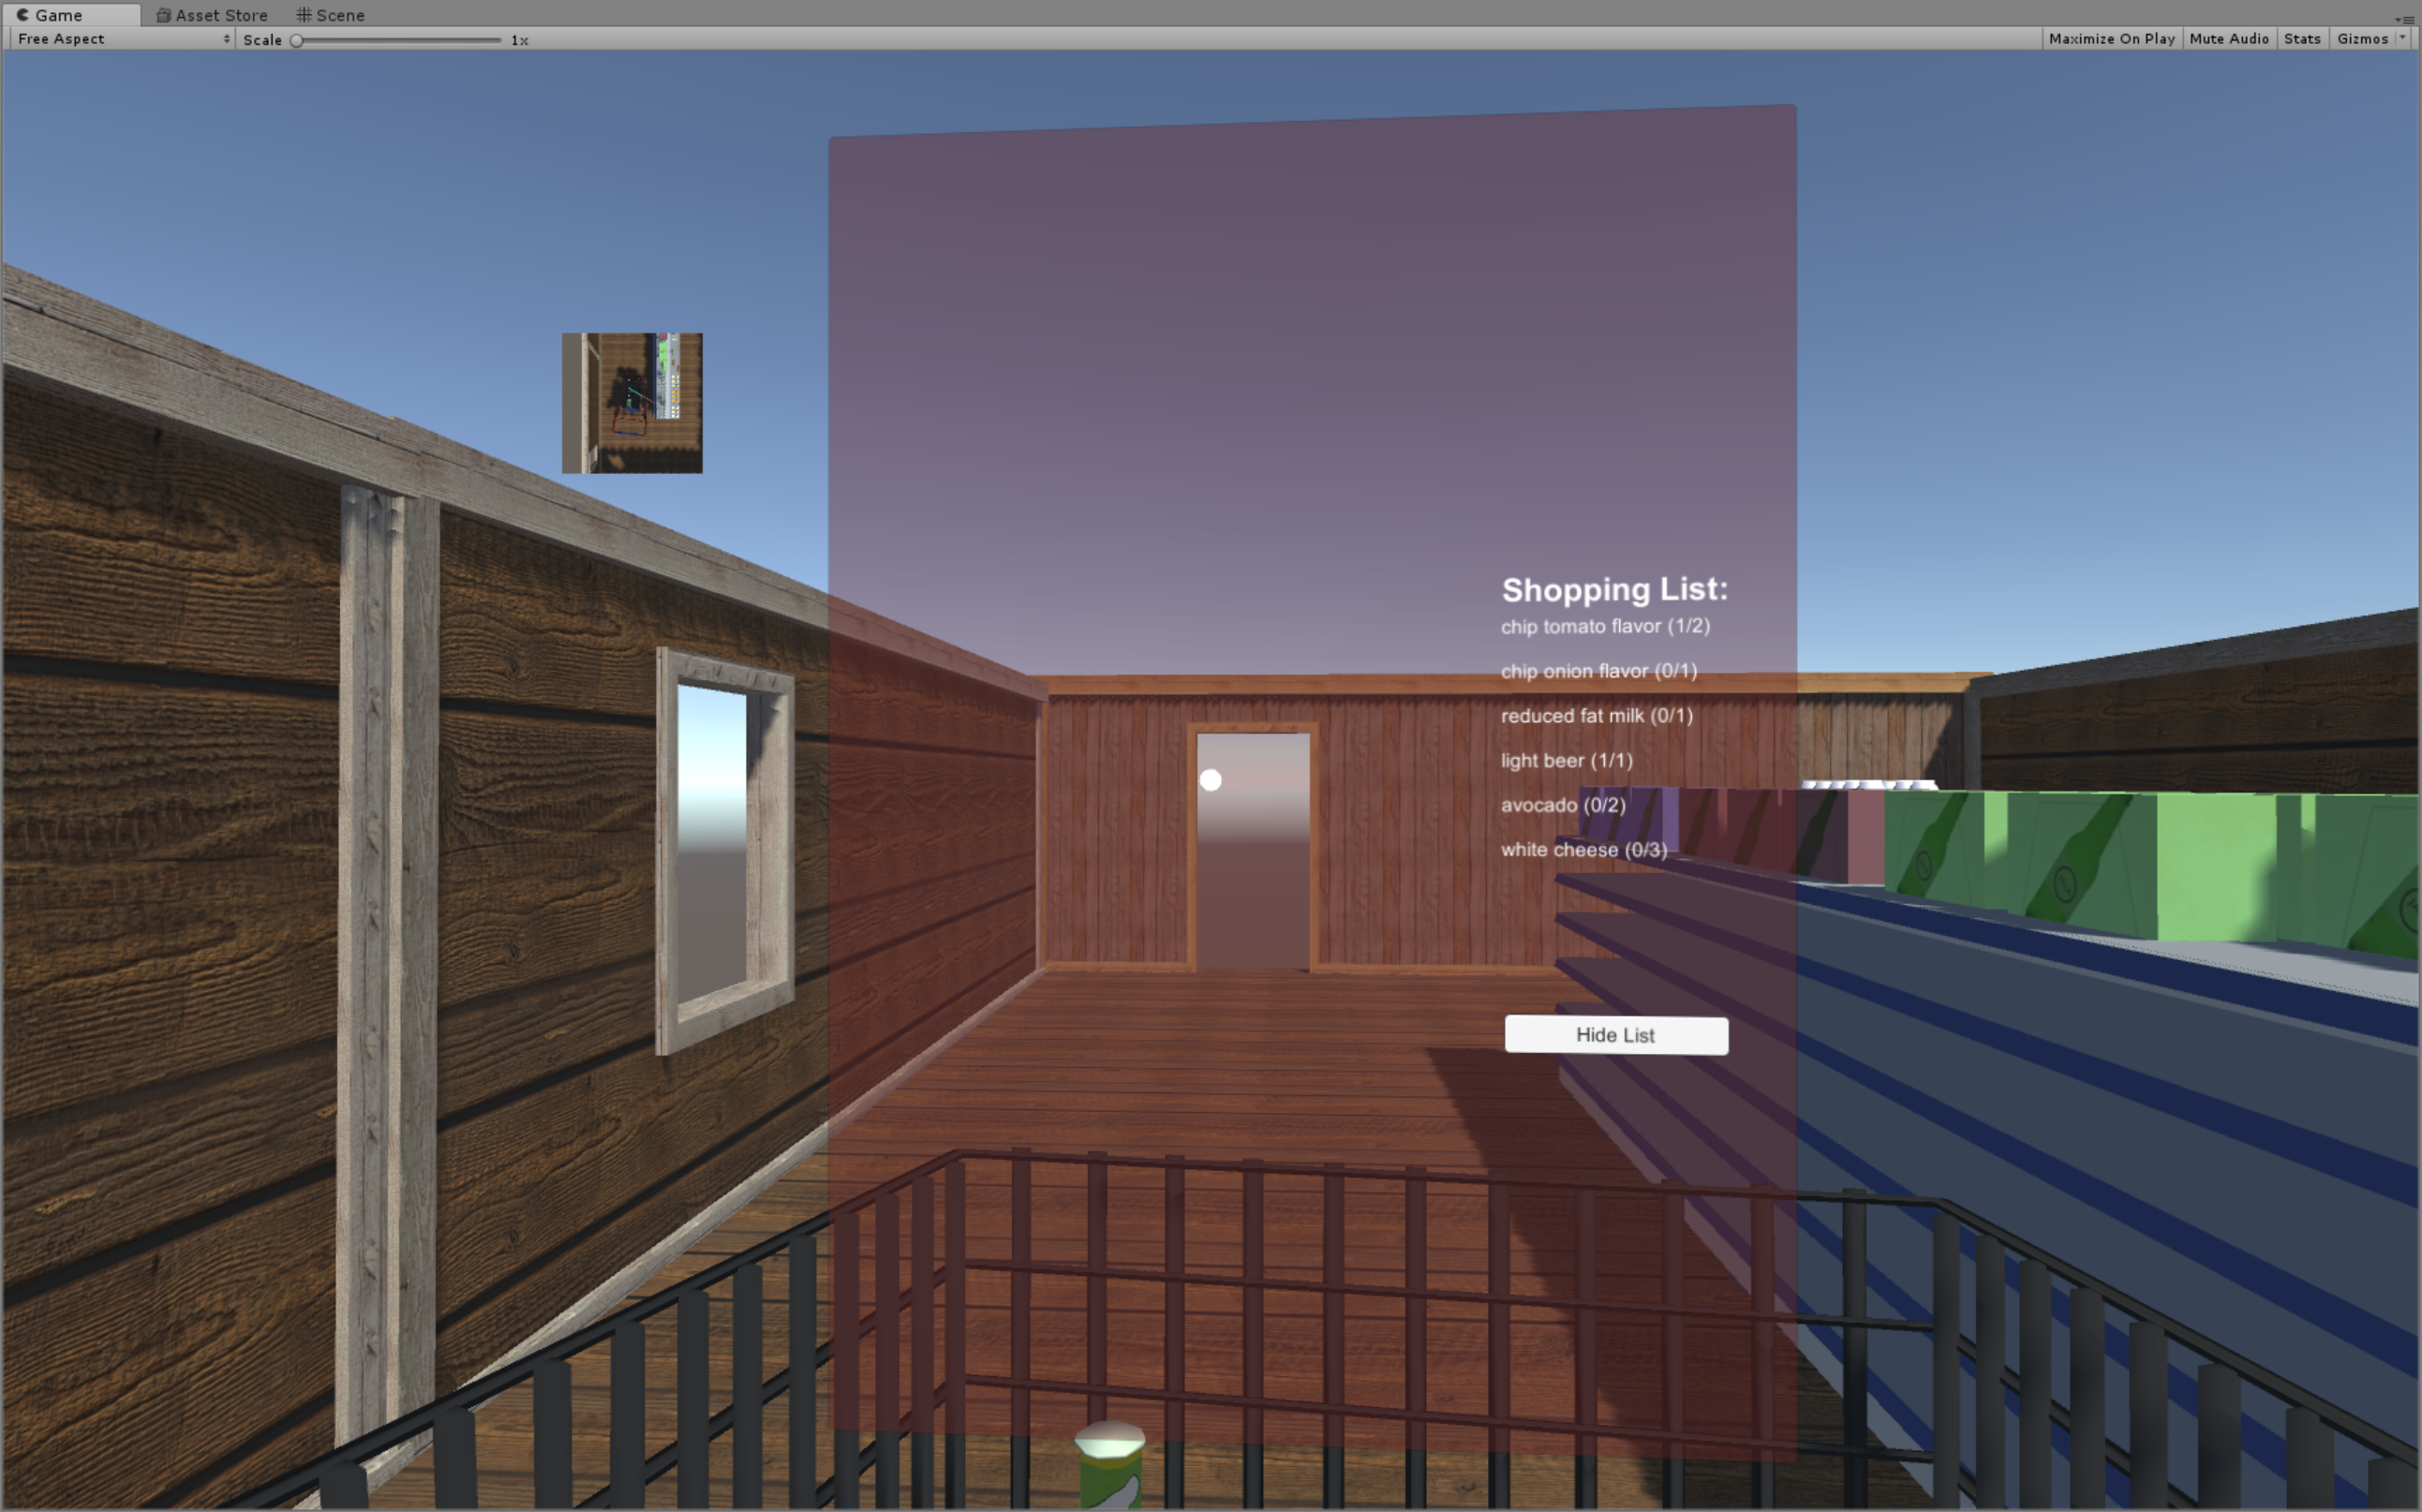
\includegraphics[width=.80\textwidth]{fig/shoppinglist.png}
		\caption{Shopping List}
	\end{figure}
	
	\subsection{Proximity Path}
	The proximity threshold is set $10$ in the virtual world. The distance is calculated directly by the locations of the cart and the original place where the item should be. If the distance is greater than the threshold, the line won't be shown.
	
	The path is displayed by an object attaching \textit{Line Renderer}. The start and the end of the path are set when the player is gazing some item on the shelf or in the cart. 
	
	\begin{figure}[htbp]
		\centering
		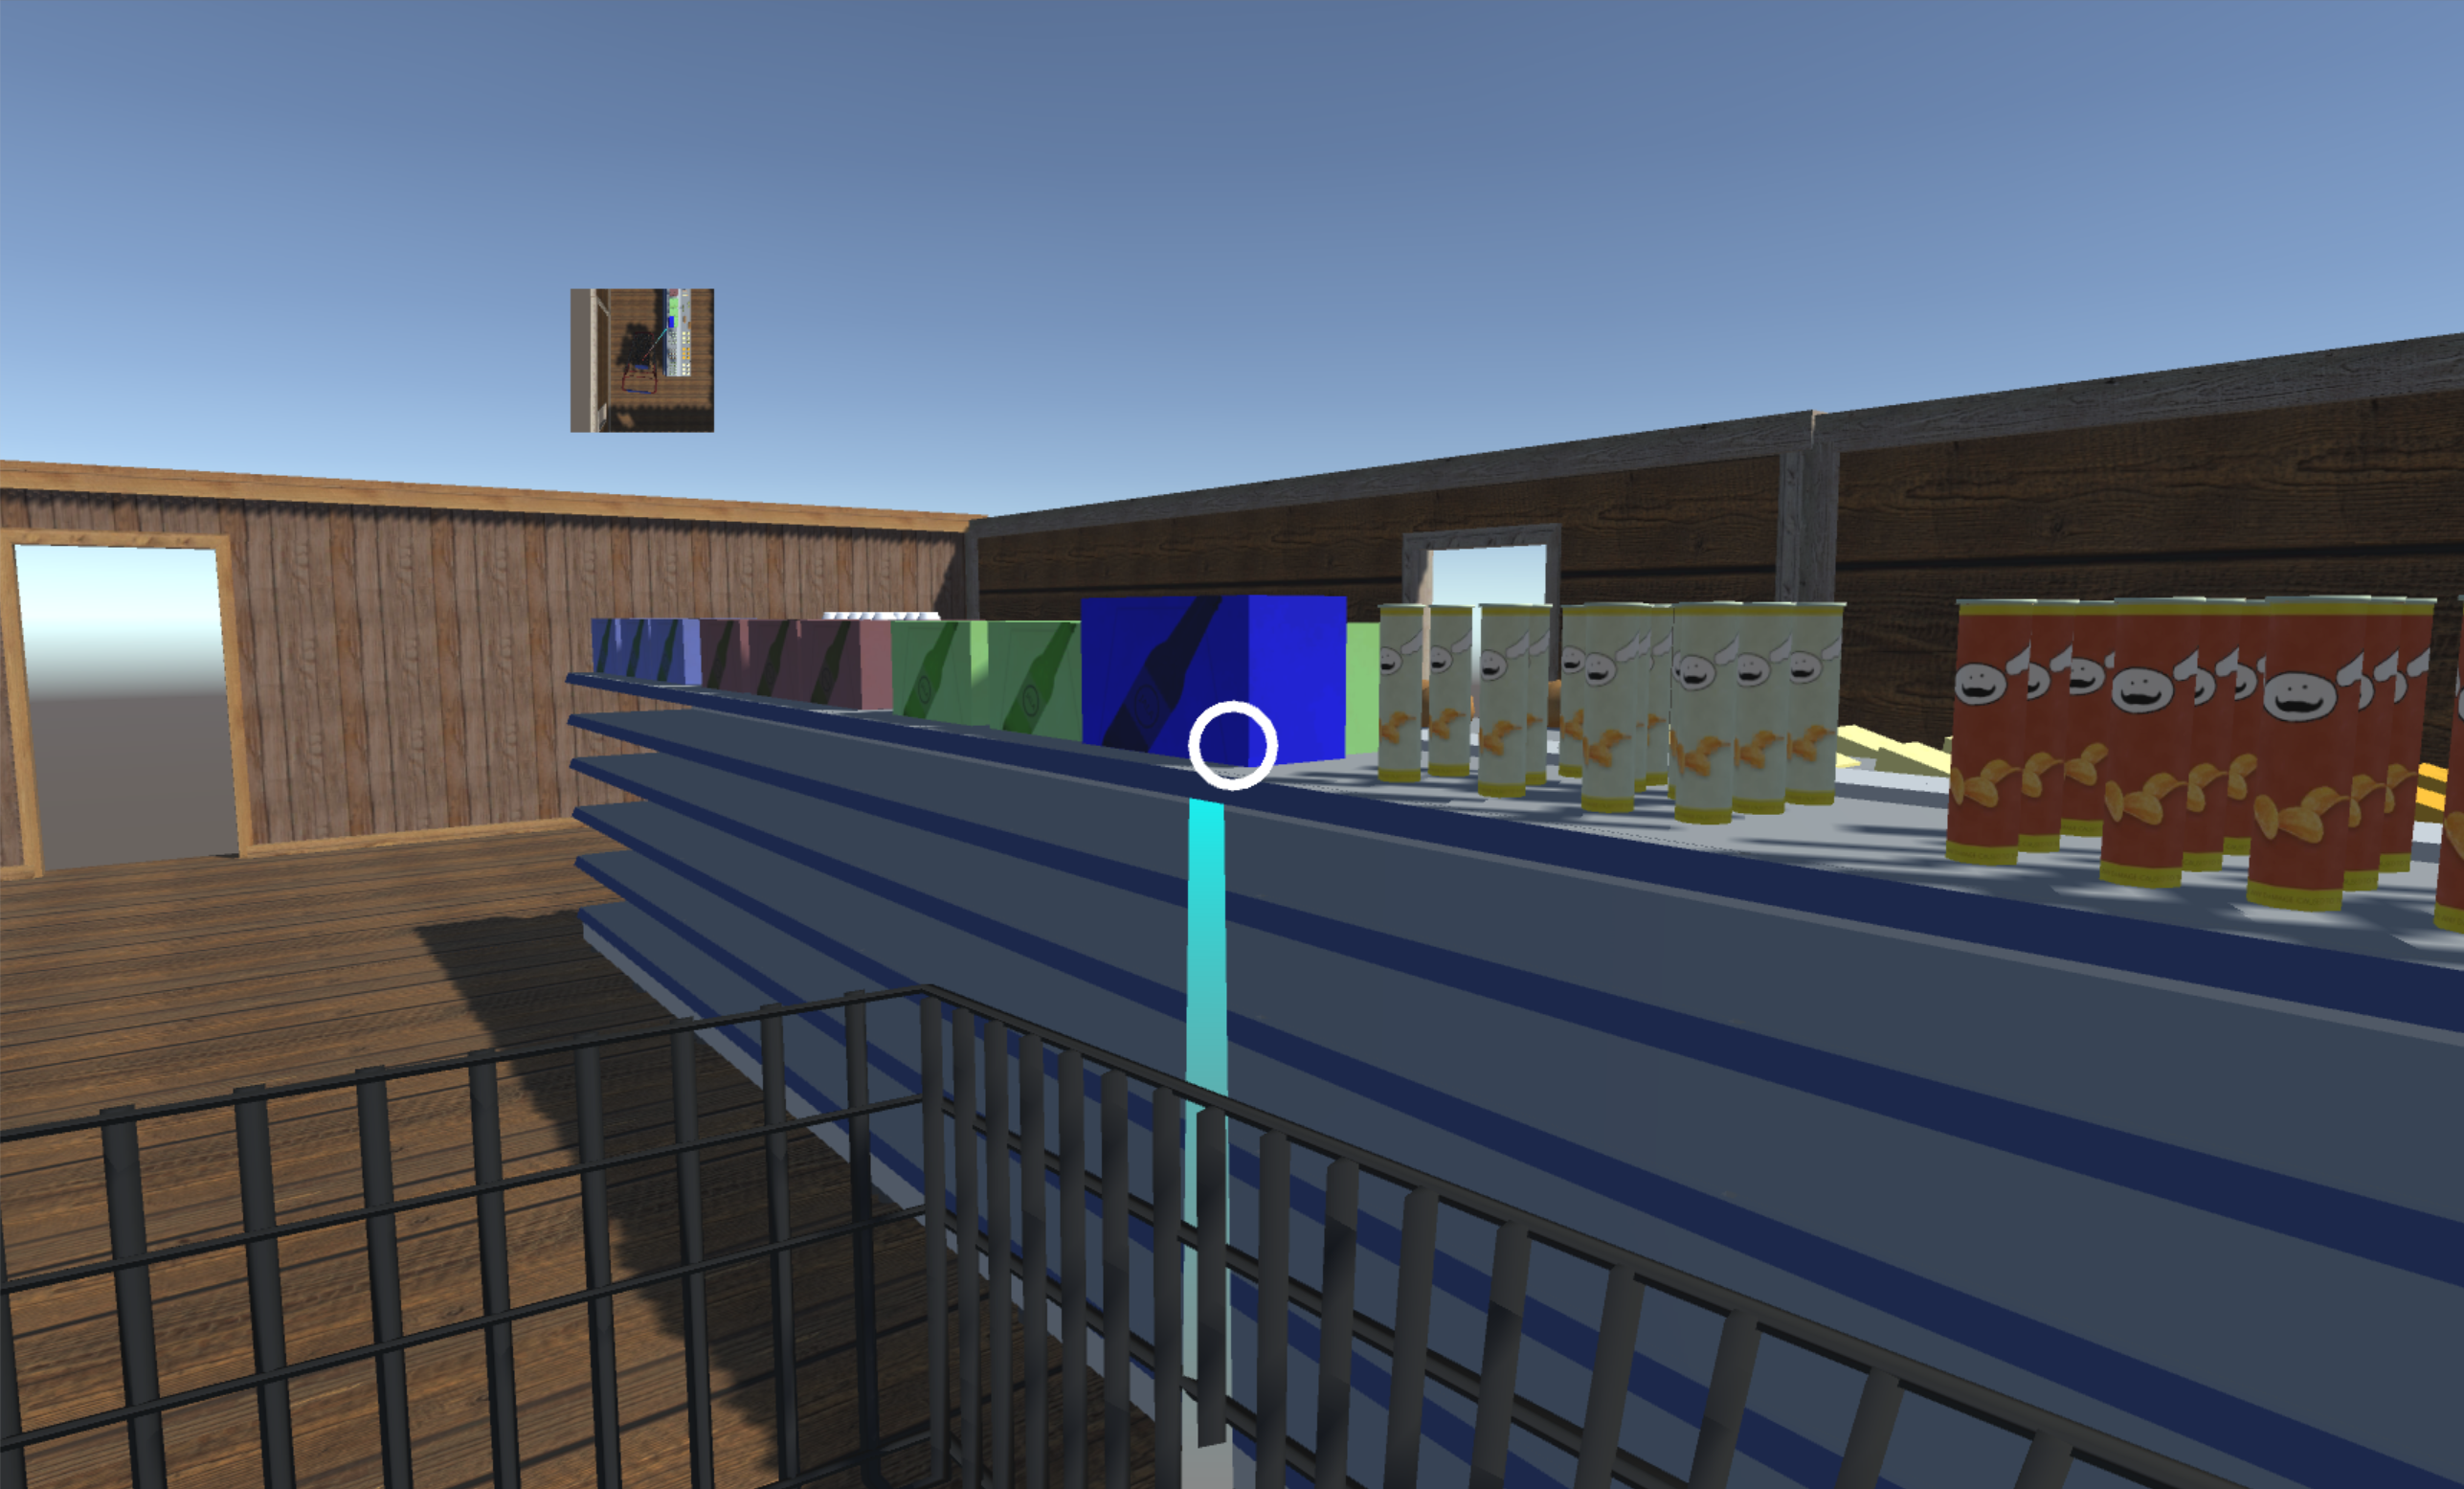
\includegraphics[width=.90\textwidth]{fig/enlargepath.png}
		\caption{Enlarging the size of the item gazed by the player}
	\end{figure}
	
	\subsection{Buy, Return and Move the Cart}
	Gaze interaction is adopted from \cite{gazeinteractiontutorial}. An item is bind by two event triggers: PointerEnter and PointerExit. These two events ensure the item to act when you are gazing. It is important to mention that the Google Cardboard SDK\cite{googlevrsdk} has already made the work that set your gaze point as a pointer. 
	
	The item will be enlarged and change its color to stress the selection.
	
	If the player is gazing at an item, when pressing $B$ on the joystick, the item will automatically move into the cart. The return can be performed by the same procedure by gazing the item in the cart.
	
	The cart is binded by 2 another keys $X$ and $Y$ on the joystick to move forward and right. Hence, in this project I use 4 keys in total to perform all the interaction features. 
	\begin{figure}[htbp]
		\centering
		\includegraphics[width=.90\textwidth]{fig/buythings.png}
		\caption{Buy Items}
	\end{figure}
	
	\subsection{Items}
	Three kinds of items are implemented into 3 different flavors/types respectively.
	\begin{figure}[htbp]
		\centering
		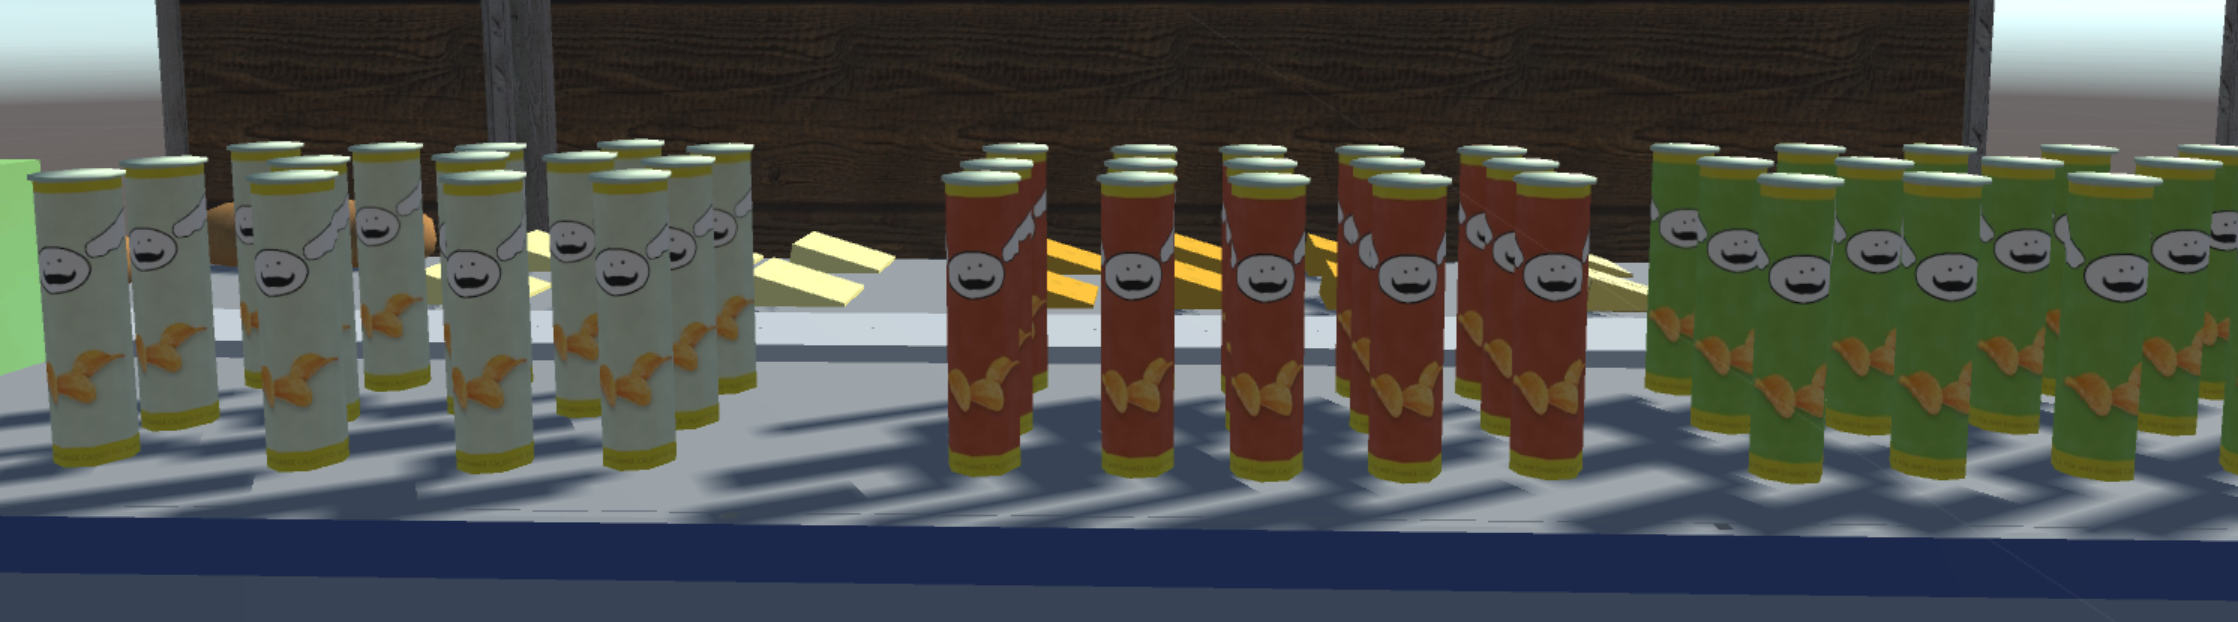
\includegraphics[width=.90\textwidth]{fig/differentflavors.png}
		\caption{Different flavors/types of items}
	\end{figure}
	
	
	\section{Acknowledgment}
	I would like to thank Xueying Bai and Ying Lu for discussions during this assignment. I also appreciate all the authors of free assets available in the Unity Asset Store.
	%\section{Findings and Results}
	%	Results are shown right in the figures, next to the figure.
	%	\begin{figure}[htbp]
	%		\centering
	%		\includegraphics[width=.90\textwidth]{fig/reselbow.png}
	%		\caption{Elbow Plot}
	%	\end{figure}
	%	\begin{figure}[htbp]
	%		\centering
	%		\includegraphics[width=.90\textwidth]{fig/resscree.png}
	%		\caption{Scree Plot}
	%	\end{figure}
	\bibliography{lab2}
	\bibliographystyle{IEEEtran}
\end{document}


